% Was a screenshot-style paste of two paragraphs from the Wayve paper, ending
% mid-sentence ("...is an experience tuple, a transition"). The application is
% worth keeping -- it is the cleanest real-robot DDPG result there is -- so the
% text is now written out rather than cropped.
\section{DDPG in the Real World}
\begin{frame}{A Real Application: Wayve --- ``Learning to Drive in a Day'' \rref{6}}
\begin{columns}[T]
\begin{column}{0.42\textwidth}
\begin{figure}
    \centering
    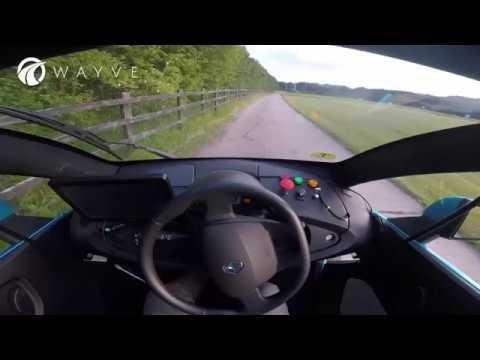
\includegraphics[width=\linewidth,height=0.62\textheight,keepaspectratio]{images/continuous-control-1/figures/wayve-car.jpg}
\end{figure}
\vspace{0.3em}
{\scriptsize A full-size car learning lane-following on a real road, from scratch. All exploration and optimisation ran on-board; a simulator was used only to tune hyperparameters beforehand.}
\end{column}
\begin{column}{0.56\textwidth}
\footnotesize
\begin{itemize}
    \setlength{\itemsep}{0.55em}
    \item \textbf{Task:} stay in lane on a real 250\,m stretch of private road. \\ \textbf{State:} a single monocular camera image. \\ \textbf{Action:} \emph{two continuous numbers} --- steering angle in $[-1,1]$ and a speed setpoint in km/h.
    \item \textbf{Reward:} forward speed. An episode ends when the safety driver intervenes, so a state's value is the distance driven before an intervention.
    \item \textbf{Result:} lane following learned in \textbf{11 episodes / 15 minutes} of real driving (35 episodes / 37 minutes when learning straight from raw pixels rather than a compressed image representation).
    \item \textbf{Why DDPG:} the authors deliberately used an \emph{off-the-shelf} algorithm with no task-specific modification, to show the problem formulation was doing the work.
    \item \textbf{Why off-policy mattered:} those few hundred metres of driving were replayed many times over. An on-policy method would have needed far more driving than a safety driver can supply.
\end{itemize}
\end{column}
\end{columns}
\end{frame}
